%
% This is a borrowed LaTeX template file for lecture notes for CS267,
% Applications of Parallel Computing, UCBerkeley EECS Department.
% Now being used for CMU's 10725 Fall 2012 Optimization course
% taught by Geoff Gordon and Ryan Tibshirani.  When preparing 
% LaTeX notes for this class, please use this template.
%
% To familiarize yourself with this template, the body contains
% some examples of its use.  Look them over.  Then you can
% run LaTeX on this file.  After you have LaTeXed this file then
% you can look over the result either by printing it out with
% dvips or using xdvi. "pdflatex template.tex" should also work.
%

\documentclass[twoside]{article}
\setlength{\oddsidemargin}{0.25 in}
\setlength{\evensidemargin}{-0.25 in}
\setlength{\topmargin}{-0.6 in}
\setlength{\textwidth}{6.5 in}
\setlength{\textheight}{8.5 in}
\setlength{\headsep}{0.75 in}
\setlength{\parindent}{0 in}
\setlength{\parskip}{0.1 in}

%
% ADD PACKAGES here:
%

\usepackage{amsmath,amsfonts,graphicx}
\usepackage{float}
\usepackage{algorithmic}
\usepackage{algorithm}
%
% The following commands set up the lecnum (lecture number)
% counter and make various numbering schemes work relative
% to the lecture number.
%
\newcounter{lecnum}
\renewcommand{\thepage}{\thelecnum-\arabic{page}}
\renewcommand{\thesection}{\thelecnum.\arabic{section}}
\renewcommand{\theequation}{\thelecnum.\arabic{equation}}
\renewcommand{\thefigure}{\thelecnum.\arabic{figure}}
\renewcommand{\thetable}{\thelecnum.\arabic{table}}

%
% The following macro is used to generate the header.
%
\newcommand{\lecture}[4]{
   \pagestyle{myheadings}
   \thispagestyle{plain}
   \newpage
   \setcounter{lecnum}{#1}
   \setcounter{page}{1}
   \noindent
   \begin{center}
   \framebox{
      \vbox{\vspace{2mm}
    \hbox to 6.28in { {\bf 10-725: Optimization
	\hfill Fall 2012} }
       \vspace{4mm}
       \hbox to 6.28in { {\Large \hfill Lecture #1: #2  \hfill} }
       \vspace{2mm}
       \hbox to 6.28in { {\it Lecturer: #3 \hfill Scribes: #4} }
      \vspace{2mm}}
   }
   \end{center}
   \markboth{Lecture #1: #2}{Lecture #1: #2}

   {\bf Note}: {\it LaTeX template courtesy of UC Berkeley EECS dept.}

   {\bf Disclaimer}: {\it These notes have not been subjected to the
   usual scrutiny reserved for formal publications.  They may be distributed
   outside this class only with the permission of the Instructor.}
   \vspace*{4mm}
}
%
% Convention for citations is authors' initials followed by the year.
% For example, to cite a paper by Leighton and Maggs you would type
% \cite{LM89}, and to cite a paper by Strassen you would type \cite{S69}.
% (To avoid bibliography problems, for now we redefine the \cite command.)
% Also commands that create a suitable format for the reference list.
\renewcommand{\cite}[1]{[#1]}
\def\beginrefs{\begin{list}%
        {[\arabic{equation}]}{\usecounter{equation}
         \setlength{\leftmargin}{2.0truecm}\setlength{\labelsep}{0.4truecm}%
         \setlength{\labelwidth}{1.6truecm}}}
\def\endrefs{\end{list}}
\def\bibentry#1{\item[\hbox{[#1]}]}

%Use this command for a figure; it puts a figure in wherever you want it.
%usage: \fig{NUMBER}{SPACE-IN-INCHES}{CAPTION}
\newcommand{\fig}[3]{
			\vspace{#2}
			\begin{center}
			Figure \thelecnum.#1:~#3
			\end{center}
	}
% Use these for theorems, lemmas, proofs, etc.
\newtheorem{theorem}{Theorem}[lecnum]
\newtheorem{lemma}[theorem]{Lemma}
\newtheorem{proposition}[theorem]{Proposition}
\newtheorem{claim}[theorem]{Claim}
\newtheorem{corollary}[theorem]{Corollary}
\newtheorem{definition}[theorem]{Definition}
\newenvironment{proof}{{\bf Proof:}}{\hfill\rule{2mm}{2mm}}

% **** IF YOU WANT TO DEFINE ADDITIONAL MACROS FOR YOURSELF, PUT THEM HERE:

\DeclareMathOperator*{\minimize}{minimize}
\DeclareMathOperator*{\tr}{tr}

\newcommand\E{\mathbb{E}}

\begin{document}
%FILL IN THE RIGHT INFO.
%\lecture{**LECTURE-NUMBER**}{**DATE**}{**LECTURER**}{**SCRIBE**}
\lecture{25}{November 27}{Ryan Tibshirani}{Matt Wytock, Supreeth Achar}
%\footnotetext{These notes are partially based on those of Nigel Mansell.}

% **** YOUR NOTES GO HERE:

\section{A Taxonomy of Optimization Methods}
In class, the general methods for minimizing function we have looked at so far are
\begin{itemize}
\item First Order Methods - Gradient descent, acceleration etc.
\item Newton's Method
\item Dual Methods - Dual Gradient Methods
\item Interior Point Methods
\end{itemize}

These four classes of methods form the basis for most of optimization. From a statistics and machine learning point of view there are a couple of important specialised methods for optimization. They aren't as broadly applicable as the general methods listed above, but when they can be used they are very useful. These specialized methods include

\begin{itemize}
\item Coordinate Descent
\item Path Algorithms
\end{itemize}

These notes look at coordinate descent, a method that can solve some classes of convex minimization problems efficiently and is highly scalable.

\section{History and motivation}

Why is it used?
\begin{itemize}
\item Very simple and easy to implement
\item Careful implementations can attain state-of-the-art
\item Scalable, e.g. don't need to keep data in memory
\end{itemize}

As we will see in the discussion for pathwise coordinate descent for lasso, it also allows us to ignore the majority of coordinates in lasso since they will be zero. Also, there are examples of coordinate descent being applied to non-convex penalties which in itself is pretty rare, see for example \cite{MFH2011}.

The idea first appeared in Fu (1998), and again in Daubechies et al. (2004), but was inexplicably ignored until three papers around 2007, and Friedman et al. (2007) really sparked interest.

\section{Coordinate-wise Minimization}

\subsection{Convex, differentiable functions}
Consider a convex, differentiable function $f:\mathcal{R}^n \rightarrow \mathcal{R}$. If at a point $\tilde{x}$, if $f(x)$ at $\tilde{x}$ is minimized along each coordinate axis, that is if we move any distance in either direction along any coordinate axis starting from the point $\tilde{x}$, the value of $f$ will be greater than or equal to the value at f. That is $$f(\tilde{x}+d\cdot e_i) \geq f(\tilde{x})$$ where $d$ is any real number and $e_i$ is the $i^{th}$ standard basis vector. 

\textbf{Assertion:} If $f$ is convex and continuous, then $\tilde{x}$ is a minimiser for the function $f$. $f(\tilde{x}) = \min_x f(x)$.
\textbf{Proof:} For a convex, continuous function the gradient is zero at the minima. The individual components of the gradient give the directions to move along each axis to reduce the function value. When all these components are zero, then moving along any coordinate axis will not decrease the function value and hence we are also at $\tilde{x}$.

\subsection{Convex, non differentiable functions}

In general, for a convex non differentiable function, coordinate wise minimization does not yield the global minimizer. For example, consider a convex function with isocontours like those shown in figure~\ref{isocontours}. At of the places where the function derivative is not smooth (like the place where the two red lines meet), the function is minimized along both coordinate axes, but these points are not minima of the function.

\begin{figure}[h!]
\label{isocontours}
\centering
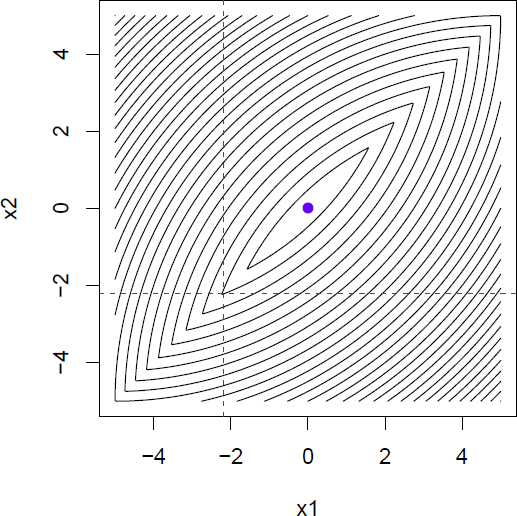
\includegraphics[width=0.5\textwidth]{images/isocontours.png}
\caption{These are the isocontours of 2D convex, non differentiable function. At the point where the two red lines meet, the function value can not be reduced by moving in either direction along either coordinate axis, but we are not at a minima of the function.}
\end{figure}

\subsection{Convex, non differentiable decomposable function}

However, if the non differentiable part of the function can be decomposed into a sum of functions over each coordinate $f(x) = g(x) + \sum_{i=1}^{n} h_i(x_i)$ where $g(x)$ is convex and smooth and each $h_i$ is convex, then the coordinate wise minimizer is the true minima of the function.

\textbf{Proof:} Consider any $x$

\begin{eqnarray}
f(x) - f(\tilde{x}) &\geq & \nabla g(x)^T(x-\tilde{x}) + \displaystyle\sum_{i=1}^{n}[h_i(x_i)-h_i(\tilde{x}_i)]\\
                    & = & \displaystyle\sum_{i=1}^n[\nabla_{i}g(\tilde{x})(x_i-\tilde{x}_i)+h_i(x_i)-h_i(\tilde{x}_i)]\\
                    & \geq & 0
\end{eqnarray}

Since $f(\tilde{x})$ is always less or equal to $f(x)$, $\tilde{x}$ must be a global minimizer of $f$.

\section{The Coordinate Descent Algorithm}

A convex, separable function of the form $f(x) = g(x) + \sum h_i(x_i)$ can be minimized by finding the coordinate wise minimizer. This point can be found from an arbitrary starting location by repeatedly cycling through coordinates and finding the value of each coordinate that minimizes the function while keeping the other coordinates fixed.

\begin{algorithm}
\caption{Coordinate Descent Algorithm}
\begin{algorithmic}
\STATE Initialize with guess $x = [x_1, x_2,...,x_n]^T $

\REPEAT{
		
	\FORALL{$j$ in $1,2,...,n$}
	\STATE $x_j \leftarrow \underset{x_j}{\text{argmin}} f(x)$
	\ENDFOR


		} \UNTIL {convergence}
\end{algorithmic}
\end{algorithm}

Points to note:
\begin{itemize}
\item The sequence of values taken on by $x$ over iterations, $x^{(k)}$ has a subsequence converging to the optimal $x^{*}$
\item $f(x^{(k)})$ converges to $f^{*}$
\item the coordinates can be cycled through in any arbitrary order
\item instead of minimizing over individual coordinates, any block of coordinates can be minimized over instead
\item however, the minimizations can not be performed in parallel, the result of one minimization must be used as the starting point for the next. The``all-at-once'' scheme is not guaranteed to converge.
\end{itemize}

For more details on the conditions for convergence and a proof refer to~\cite{T01}.

\section{Applications of Coordinate Descent}
Here are some problems that can be solved using coordinate descent

\subsection{Linear Regression}

Consider the standard linear regression problem. Find x to minimize $f(x) = \dfrac{1}{2}||y-Ax||^2$, with $y \in \mathcal{R}^n$ and $A \in \mathcal{R}^{n\times p}$. Let $A_1, A_2, ..., A_p$ denote the columns of A.
To minimize over a single coordinate $x_i$ in $x$ with all over values in $x$ fixed we have
\begin{eqnarray*}
\nabla_i f(x) &= & 0           \\
              & = & A_i^T(Ax-y)\\
              & = & A_i^T(A_ix_i + A_{-i}x_{-i}-y) \\
\end{eqnarray*}

Where $A_{-i}$ is the matrix obtained by deleting column $i$ from $A$. This equation can  be solved for $x_i$.

\begin{equation*}
x_i = \frac{A_i^T(y-A_{-i}x_{-i})}{A_i^TA_i} = \frac{A_i^Tr}{||A_i||^2} + x_i^{old}
\end{equation*}

Where $r = y-Ax$. Coordinate descent can be performed by cycling through all values of $i$ and solving the above equation for each element $x_i$. Computationally, each coordinate descent update takes $\mathcal{O}(n)$ time and so running through a full cycle over all the coordinates will take $\mathcal{O}(np)$ time. This is the same amount of time as one iteration of gradient descent. Coordinate descent is often faster than gradient descent for linear regression problems (see figure~\ref{cgvsgd}), ie it converges to the correct solution in fewer iterations. In fact, it is even faster than accelerated gradients. Accelerated gradient descent is an optimal first order method, but coordinate descent uses more than first order information.

\begin{figure}[h!]
\label{cgvsgd}
\centering
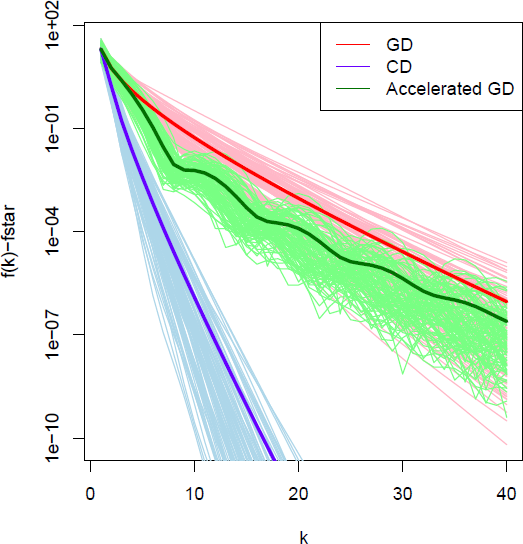
\includegraphics[width=0.5\textwidth]{images/cd_vs_gd.png}
\caption{A comparison of coordinate descent (blue), gradient descent (red) and accelerated descent (green) on 100 random instances of a linear regression problems ($n = 100$, $p = 20$).}
\end{figure}

\subsection{Lasso Regression}

For $L1$ regularized version of the regression problem $f(x) = \frac{1}{2}||y-Ax||^2+\lambda ||x||_1$. The regularizer is non smooth, but it is separable - $||x||_1 = \sum |x_i|$. Following the same approach of minimizing over $x_i$ while keeping all other coordinates fixed we get the following update rule

\begin{equation*}
x_i = S_{\lambda / ||A_i||^2}\left(\frac{A_i^T\left(y-A_{-i}x_{-i}\right)}{A_i^TA_i}\right)
\end{equation*}

where $S_\alpha$ is the soft thresholding function with parameter $\alpha$.

\subsection{Box Constrained Regression}

We want to perform linear regression given the constraint that for all $i$ $-s \leq x_i \leq s$.

\begin{equation*}
\begin{aligned}
& \displaystyle \min_{x \in \mathcal{R}^n} & \frac{1}{2}||y-Ax||^2 \\ 
& \text{subject to}                        & ||x||_{\infty} \leq s \\
\end{aligned}
\end{equation*}

By minimizing over $x_i$ while keeping all other coordinates fixed we get the update rule

\begin{equation*}
x_i = T_s\left( \frac{A_i^T\left(y-A_{-i}x_{-i}\right)} {A_i^TA_i} \right)
\end{equation*}

$T_s$ is the truncating operator whose value is the same as the input between $-s$ and $+s$, equal to $s$ for inputs greater than $s$ and equal to $-s$ for inputs less than $-s$.

\subsection{Support Vector Machines}

The dual formulation of the support vector machine optimization problem is

\begin{equation*}
\begin{aligned}
& \displaystyle \min_{\alpha \in \mathcal{R}^n} & \frac{1}{2}\alpha^TK\alpha - 1^T\alpha \\ 
& \text{subject to}                             & 0 \leq \alpha \leq C                   \\
&												& y^T\alpha = 0
\end{aligned}
\end{equation*} 

The $y^T\alpha = 0$ constraint is non separable, but it can still be shown that a coordinate descent strategy called sequential minimal optimization (SMO) can solve the problem. The complementary slackness conditions for the primal are

\begin{equation*}
\begin{aligned}
\alpha_i[(Av)_i - y_id - (1-s_i)] &=& 0 & \quad & i=1,...,n \\
(C-\alpha_i)s_i                   &=& 0 & \quad & i=1,...,n \\
\end{aligned}
\end{equation*}

where $v$ is the primal coefficients, $d$ is the primal intercept and $s$ is a vector of slacks. SMO works over blocks of two coordinates at a time. Pairs of coordinates that do not satisfy the complementary slackness conditions are chosen and jointly optimized over while respecting the $y^T\alpha = 0$ constraint and the complementary slackness constraint pair for the two variables. This 2 element block minimization step reduces to minimizing a quadratic over a line segment. Instead of chosing coordinate pairs sequentially, SMO picks the next pair to optimize over greedily using heuristics.

For more information on the SMO method including choice of heuristics, block minimization and convergence proofs refer to~\cite{P98}. 

\subsection{Graphical Lasso}

\begin{figure}
\begin{center}
\hspace{.5in}
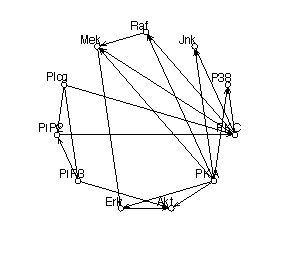
\includegraphics{images/glasso1}
\hfill
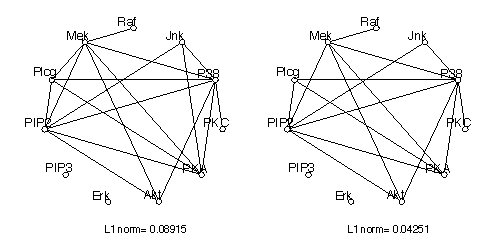
\includegraphics{images/glasso2}
\end{center}
\caption{Graphical lasso example, the true graph (left) and estimated graphs (right).}
\label{glasso}
\end{figure}

This is the application of coordinate descent to a problem that is ``pretty hard to solve'' in general. Given a matrix $A \in \mathbb{R}^{n \times p}$ of $n$ observations from a $p$-dimensional multivariate Gaussian, $\mathcal{N}(0,\Sigma)$, we want to estimate the unknown covariance matrix $\Sigma$. 

For a Gaussian distribution, we have $\Sigma_{ij}^{-1} = 0$ if and only if variables are $i$ and $j$ are conditionally independent given the other variables. Note that in the language of graphical models, this is referred to as a Gaussian Markov random field and the problem of estimating the inverse covariance is equivalent to estimating the edges between the nodes in this graph. For an example from \cite{FHT07}, see Figure \ref{glasso}.

Under a zero-mean Guassian distribution, we can formulate the $\ell_1$ penalized maximum likelihood problem as 
\begin{equation*}
\minimize_{\Theta \in \mathcal{R}^{p \times p}} -\log \det \Theta + \tr S \Theta + \lambda \|\Theta \|_1
\end{equation*}
where $S$ is the empirical covariance matrix, $S = \frac{1}{n}A^TA$.  Its straightforward to see that that stationarity KKT conditions are given by 
\begin{equation*}
-\Theta^{-1} + S + \lambda\Gamma = 0
\end{equation*}
where $\Gamma_{ij} \in \partial|\Theta_{ij}|$. Let $W = \Theta^{-1}$ and then partition the matrix blockwise
\begin{align*}
W = \left[ \begin{array}{ll} W_{11} & w_{12} \\ w_{21} & w_{22} \end{array} \right] &&
\Theta = \left[ \begin{array}{ll} \Theta_{11} & \theta_{12} \\ \theta_{21} & \theta_{22} \end{array} \right] &&
S = \left[ \begin{array}{ll} S_{11} & s_{12} \\ s_{21} & s_{22} \end{array} \right] &&
\Gamma = \left[ \begin{array}{ll} \Gamma_{11} & \gamma_{12} \\ \gamma_{21} & \gamma_{22} \end{array} \right]
\end{align*}
where $W_{11} \in \mathbb{R}^{(p-1)\times(p-1)}$, $w_{12} \in \mathbb{R}^{(p-1)\times 1}$, $w_{21} \in \mathbb{R}^{1\times(p -1)}$, and $w_{22} \in \mathbb{R}$.  This allows us to solve for a single row (or column---doesn't matter due to symmetry) while holding the others fixed. Note that for the diagonal elements of $W$, we have $W_{ii} = S_{ii} + \lambda$ because we have $\Theta_{ii} > 0$ at the solution. Therefore, we solve for $w_{12}$, and then cycle through the columns by holding the other ones fixed, etc.

Considering the just $(1,2)$ block of the KKT conditions we have
\begin{equation*}
-w_{12} + s_{12} + \lambda\gamma_{12} = 0
\end{equation*}
Because
\begin{equation*}
\left[ \begin{array}{ll} W_{11} & w_{12} \\ w_{21} & w_{22} \end{array} \right]\left[ \begin{array}{ll} \Theta_{11} & \theta_{12} \\ \theta_{21} & \theta_{22} \end{array} \right] = 
\left[ \begin{array}{ll} I & 0 \\ 0 & 1 \end{array} \right]
\end{equation*}
we have $w_{12} = -W_{11}\theta_{12}/\theta_{22}$, which we can subsitute back into the above equation to get
\begin{equation*}
W_{11}\frac{\theta_{12}}{\theta_{22}} + s_{12} + \lambda\gamma_{12} = 0
\end{equation*}
But letting $x = \theta_{12}/\theta_{22}$ and noting that $\theta_{22} > 0$ at the solution, this can be written as 
\begin{equation*}
W_{12}x + s_{12} + \lambda \rho = 0
\end{equation*}
where $\rho \in \partial \|x \|_1$ which is exactly the KKT conditions for
\begin{equation*}
\minimize x^TW_{11}x + s_{12}^Tx + \lambda \|x\|_1
\end{equation*}
which is a lasso problem that can be solved quickly via coordinate descent. So in summary we can solve the graphical lasso problem by applying coordinate descent to get a series of lasso problems.

Note that by reparameterizing in terms of $W$, and then solving in terms of blocks of $W$, these \emph{do not} correspond to blocks $\Theta$ so this is not technically a coordinate descent algorithm. However, there is a nice result from Mazumder et al. \cite{MH11} that shows that this is actually performing coordinate ascent in the dual problem so everything is okay.

\section{Pathwise coordinate descent for lasso}

Here we exploit sparsity in the in the problem to make the algorithm more efficient. 

Outer loop:
\begin{itemize}
\item Compute the solution at sequence $\lambda_1 \ge \lambda_2 \ge \ldots \ge \lambda_r$
\item For $\lambda_k$, initialize coordinate descenta lgorithm at the compute solution for $\lambda_{k+1}$ (warm start)
\end{itemize}

Inner loop:
\begin{itemize}
\item Perform one (or a small number) of complete cycles and record the active set $S$ of coefficients that are nonzero
\item Cycle over coefficients $S$ until convergence
\item Check KKT conditions over all coefficients; if not all satisified, add offending coefficients to $S$ and go back one step
\end{itemize}

With these strategies in place, coordinate descent is competitive with fastest algorithms for lasso problems. Freely available in the ``glmnet'' package in MATLAB and R.

\section{No convergence rates}

There is a dearth of theory for coordinate descent especially when it comes to convergence rates---theory is sorely needed. In general, we do not have global convergence rates. In recent work, Saha et al. \cite{ST10} consider a restricted class of problems
\begin{equation*}
f(x) = g(x) + \lambda \|x\|_1
\end{equation*}
with $g$ convex. However, they assume that
\begin{itemize}
\item $\nabla g$ Lipschitz with constant $L > 0$ and $I - \nabla g/L$ montone increasing in each component
\item there is a $z$ such that $z \ge S_\lambda(z - \nabla g(z))$ or $z \le S_\lambda(z - \nabla g(z))$
\end{itemize}
The first condition is ``a little bit funny.'' A sufficient condition for this is that the off-diagonal elements of the Hessian of $g$ at any $x$ are nonpositive. The second condition follows from the first condition, as is shown in the paper.

They show that for coordinate descent starting at $x^{(0)} = z$ and generalized gradient descent starting at $y^{(0)} = z$ with step size $1/L$, we have
\begin{equation*}
f(x^{(k)}) - f(x^\star) \le f(y^{(k)}) - f(x^\star) \le \frac{L\|x^{(0)} - x^\star\|^2}{2k}
\end{equation*}
In other words, coordinate descent dominates generalized gradient descent at every iteration. It's not clear if this fully explains the behavior that we see in practice or how big this class of problems is due to the assumptions.

\section*{References}
\beginrefs
\bibentry{FHT07} J. Friedman, T. Hastie and R. Tibshirani, ``Sparse inverse covariance estimation with the graphical lasso.''
\bibentry{MH11} R. Mazumder and T. Hastie, ``The graphical lasso: new insights and alternatives.''
\bibentry{MFH11} R. Mazumder, J. Friedman and T. Hastie, ``SparseNet: coordinate descent with non-convex penalties''
\bibentry{P98} J.~Platt, ``Sequential Minimal Optimization: A Fast Algorithm for Training Support Vector Machines,'' {\it Advances in Kernel Methods}, pp.~185-208.
\bibentry{ST10} A. Saha and A. Tewari, ``On the finite time convergence of cyclc coordinate descent methods.''
\bibentry{T01} P.~Tseng, ``Convergence of Block Coordinate Descent Method for Nondifferentiable Minimization,'' {\it Journal of Optimization Theory and Applications}, Vol 109, Issue 3.
\endrefs

% **** THIS ENDS THE EXAMPLES. DON'T DELETE THE FOLLOWING LINE:

\end{document}





